%!TEX root=../../../main.tex

While annotations facilitate individual note taking for users and improve
engagement inside platforms deploying such mechanisms, it is also desirable
that metadata can be shared across ecosystems in order to allow for new
connections between information resources to be discovered. Thus, the usage of
standard annotation dissemination formats is necessary.

The systems presented in the previous subsection make use of different forms of
RDF structures in order to represent annotations both internally and
externally.  RDF, or the Resource Description Framework \cite{ref:rdf} is a
model defined by the World Wide Web Consortium (W3C) to be used for online data
interchange. The main idea behind it is related to making statements about
resources in the form of subject-predicate-object expressions, such as:

\begin{verbatim}
  <Dave Beckett> <edits> <the RDF syntax grammar specification>
\end{verbatim}

Due to their structure, these statements are named \textit{triples} in the RDF
terminology.  A collection of RDF statements will constitute a directed
multi-graph, also named the \textit{context} of the concerned triples. A simple
example is shown in Fig. \ref{fig:rdf}

\begin{figure}[!h]
  \centering
  \fbox{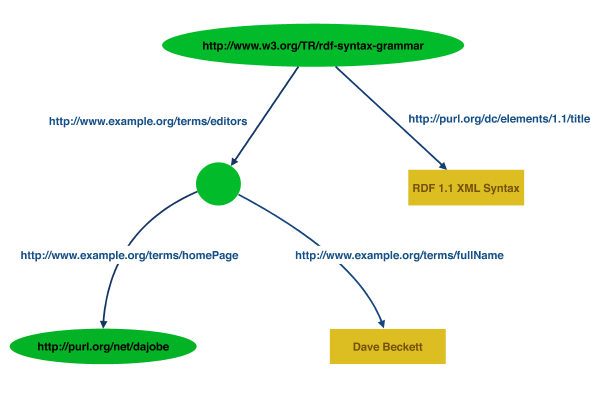
\includegraphics[scale=1]{static/img/rdf.png}}
  \caption[Example RDF graph]
          {Example RDF graph, source \cite{ref:rdfsyntax}. Briefly, this graph
           can be summarised as: The RDF syntax specification, identified by a
           URL, has a person identified by its full name and personal Web page
           as an editor.}
  \label{fig:rdf}
\end{figure}

It can be observed that this model is very well-suited for the annotations use
case. Metadata can be seen as a statement about a resource in the form (but
not restricted to):

\begin{verbatim}
  <Resource identified by URL/ URI> <has metadata> <annotation body text>
\end{verbatim}

The RDF data model can be serialised in different formats, such as Turtle,
N-Triples, N-Quads (a superset of N-Triples), Notation 3 (N3), RDF/XML or
JSON-LD. Note that the RDF/XML format is commonly referred to simply XML, due
to its widespread usage, leading to some confusion between the \textit{data
  model} and the \textit{serialisation format}. A typical RDF/XML document will
look as the one in Listing \ref{lst:rdf}, which encodes the graph in Fig.
\ref{fig:rdf}. In order to be encoded in XML, the RDF graph nodes
and predicates need to be represented in the specific XML structural terms:
element and attribute names, element contents and attribute values. Note that
the example XML uses three collections to define the elements, namely the RDF
standard set, the Dublin Core Metadata Element Set \cite{ref:dc} and a
placeholder set; in real use-cases, each Web application can define its own set
of elements, depending on the specific domain knowledge.

\begin{figure}[!h]
  \lstinputlisting[language=XML,
                   frame=tb,
                   captionpos=b,
                   numbers=none,
                   showspaces=false,
                   showstringspaces=false,
                   showtabs=false,
                   stepnumber=2,
                   numbersep=4pt]
    {static/lst/rdf.xml}
    \caption[RDF/XML Example]
            {RDF/XML Example, source \cite{ref:rdfsyntax}}
    \label{lst:rdf}
\end{figure}

Similar to the RDF/XML, an augmented version of the JavaScript Object Notation
(JSON) format, JSON-LD, can also be used to serialize the data model; an
in-detail description, in the usage context of the project is included in
Section \ref{sec:json}.

Relational databases, while not suitable for the graph structure of the RDF
model, are the most used solution for storing such data. If a database stores
only the triples it is called a \textit{triplestore}, and if the context is
also included, a \textit{quad} store is employed. These stores can be queried
using the SPARQL \cite{ref:sparql} query language.

While RDF provides a standard method for disseminating data, it is mainly
purposed for machine consumption. Taking the RDF/XML format as an example, it
can be seen that edditing such a format by hand is not optimal for end-users.
On the other hand, capturing input and filling an XML template, while
accounting for invalid data or out-of-scope information, can become expensive
in terms of computing resources.

A simple solution is to deploy standard forms for guiding the users in the data
colelction process. The Pundit project discussed previously uses such a form for
allowing users to input RDF statements. While this solution is fast to develop
due to the prevalence of the practice in Web applications, it also lack in terms
of extendability and scalability; it can be seen that in order to be able to
express complex RDF graphs, a considerable effort must be invested.

The XTiger \cite{ref:xtiger} XML language allows defining templates, in order
to guide an editting tool for building documents that follow a predefined
model. It does this by predefining a set of typed structures and constructors
for these (\textit{components}); for example, a minimal annotation template
could be defined as in Listing \ref{lst:xtiger}. The XTiger template can be
used to generate documents in a target language, for example XHTML.

\begin{figure}[!h]
  \lstinputlisting[language=XML,
                   frame=tb,
                   captionpos=b,
                   numbers=none,
                   showspaces=false,
                   showstringspaces=false,
                   showtabs=false,
                   stepnumber=2,
                   numbersep=4pt]
    {static/lst/xtiger.xml}
    \caption[XTiger template fragment for annotations]
            {Minimal XTiger template for annotations. It defines two components
             that construct the fields that must be filled in by the end-user.
             The components can be used in the document body for producing
             a form, the target language being XHTML.}
    \label{lst:xtiger}
\end{figure}

Special constructs for repeating components accross the resulting document can
ease the creation of complex structures. RDF graphs can be constructed by using
the RDF/XML serialisation format as the target for a XTiger template and by
leveraging the special contructs (e.g., \texttt{xt:repeat}) that allow
repeating components accross the produced document. To allow even further
flexibility, the Adaptable XML Editing Library (AXEL) \cite{ref:axel} can be
used. This JavaScript library allows users to freely combine template
components, while still producing conforming documents as the end-result.
